\chapter{Анализ методов повышения качества на границе проводной и беспроводной сети} \label{chapt1}


\section{Анализ перспектив развития беспроводных сетей} \label{sect1_0}
В этом разделе мы расмотрим тендеции развития мобильной связи.
Согласно отчета Ericsson \cite{ericsson} число абонентов мобильной связи во всем мире выросло примерно на 8 процентов в годовом исчислении в 1 квартале 2013 года. Число абонентов подвижной широкополосной связи выросло еще быстрее за этот период в размере 45 процентов в годовом исчислении, достигнув около 1,7 миллиарда. Количество данных, передаваемые каждым усстройством, также неуклонно продолжают расти. Около 50 процентов всех проданных мобильных телефонов в 1 квартале 2013 были смартфонами. Все эти фактроры привели к удвоению мобильного трафика между 1 кварталом 2012 и 1 кварталом 2013 года. 

В 1 квартале 2013 года общее количесво мобильных устройств превысило 6,4 миллиарда. К концу 2018 года ожидается 9,1 миллиард обслуживаемых устройств. 

Глобальное количество обслуживаемых широкополосных устройств достигло в 1 квартал 2013 года 1,7 миллиарда и к концу 2018 года достигнет 7 миллиардов (рис. \ref{img1:mob1}). Основными устройствами шрокополосного доступа есть и будут продолжать быть смартфоны. Мобильный широкополосный доступ получит большую долю от общей широкополосной связи на многих рынках, дополняя XDSL в определенных сегментах и заменяя его в других. 

Количество обслуживаемых мобильных устройств, таких как мобильные ПК, мобильные роутеры, планшеты, которые используют большой экран, увеличится с 300 млн в 2012 году до 850 млн в 2018 году, что привысит число абонентов фиксированной широкополосной связи (рис. \ref{img1:mob2}).
Общее количество смартфонов достигло в 2012 году 1,2 млрд и, как ожидается, вырастет до 4,5 млрд в 2018 году. На сегодняшний день основным мобильным устройсвом является базовый телефон. Проникновение смартфонов будет быстро увеличиваться, в то время как, по оценкам, количество обслуживаемых базовых телефонов останется высоким, медленно снижаясь с 5 млрд сегодня до 4 млрд в 2018 году. Это связано с тем что базовые телефоны будут продолжать находится в нижнем сегменте продаваемых абонентских устройств.
\begin{figure} [h]
  \center
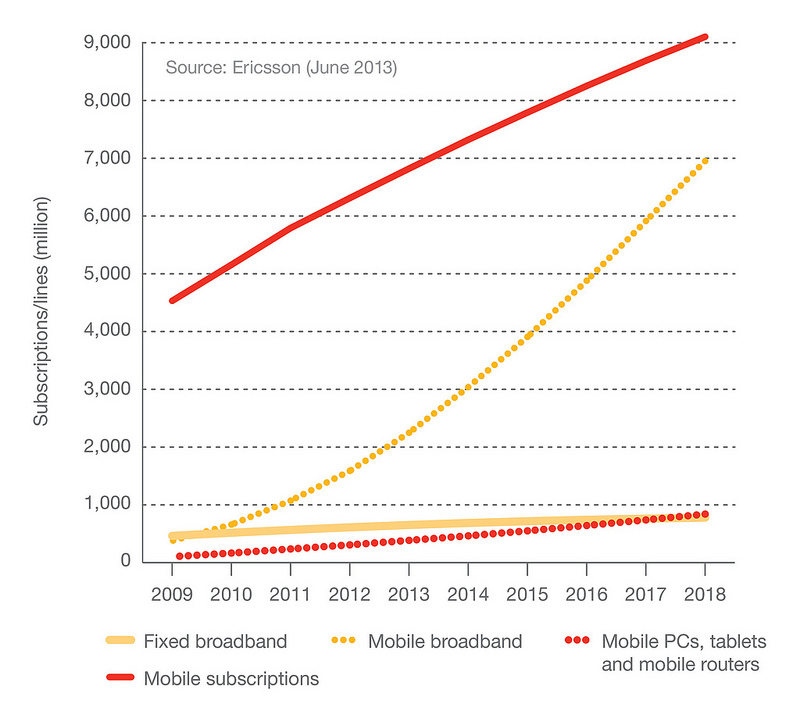
\includegraphics[width=0.8\textwidth]{ericsson/mob1.png}
  \caption{Стационарные и мобильные обслуживаемые устройства, 2009-2018 \cite{ericsson}}
  \label{img1:mob1}
\end{figure}


\pgfplotsset{width=15cm, height=10cm, compat=1.3}
\begin{figure} [h]
  \center
\begin{tikzpicture}
\pgfkeys{ /pgf/number format/.cd,
        use comma,
        1000 sep={}}
\pgfkeys{/pgfplots/legend pos=north west}



\begin{axis}[stack plots=y,/tikz/ybar,
xlabel=Год,
ylabel=Абонентов (млн)
]
\addplot coordinates
{(2010,4466) (2011,4711) (2012,4741) (2013,4639) (2014,4483) (2015,4289) (2016,4099) (2017,3926) (2018,3763)};
\addplot coordinates
{(2010,522) (2011,836) (2012,1247) (2013,1781) (2014,2363) (2015,2944) (2016,3504) (2017,4017) (2018,4493)};
\addplot coordinates
{(2010,166) (2011,238) (2012,308) (2013,386) (2014,467) (2015,554) (2016,647) (2017,745) (2018,846)};

\legend{Функциональный/Базовый телефон, Смартфон, Мобильный ПК/Маршрутизатор/Планшет}
\end{axis}
\end{tikzpicture}
\caption{Прогноз развития беспроводных сетей по устройствам от \cite{ericsson}}
  \label{img1:mob2}
\end{figure}


\clearpage


На рис. \ref{img1:mob3} иллюстрирован отчет по количеству обслуживаемых мобильных устройств разбитых по технологиям. LTE, которое развернуто и представлено во всех регионах, в 2018 году составит 2 млрд устройств. Эти устройства будут представлять лидирующую долю от обшего количества устройств. Быстрый переход на более совершенные технологии в развитых странах, означает что глобально количество абонентов GSM/EDGE будет снижаться после 2012-2013 годов. Глобально, GSM/EDGE будет продолжать играть ведущую роль с точки зрения числа абонентов до послених лет прогнозного периода. Это связано с тем что новые менее обеспеченные пользователи, вероятно будут использовать самые дешовые мобильные устройства и технологии мобильной связи. Кроме этого требуется время для обновления установленной базы мобильных устройств.


\pgfplotsset{width=15cm, height=10cm, compat=1.3}
\begin{figure} [h]
  \center
\begin{tikzpicture}
\pgfkeys{ /pgf/number format/.cd,
        use comma,
        1000 sep={}}
\pgfkeys{/pgfplots/legend pos=north west}
\begin{axis}[stack plots=y,/tikz/ybar,
xlabel=Год,
ylabel=Абонентов (млн)
]
\addplot coordinates
{(2010,64) (2011,54) (2012,37) (2013,34) (2014,35) (2015,35) (2016,35) (2017,29) (2018,23)};
\addplot coordinates
{(2010,497) (2011,532) (2012,545) (2013,537) (2014,525) (2015,514) (2016,503) (2017,485) (2018,473)};
\addplot coordinates
{(2010,21) (2011,51) (2012,94) (2013,149) (2014,199) (2015,229) (2016,231) (2017,223) (2018,201)};
\addplot coordinates
{(2010,3904) (2011,4182) (2012,4311) (2013,4263) (2014,4060) (2015,3717) (2016,3240) (2017,2696) (2018,2117)};
\addplot coordinates
{(2010,668) (2011,956) (2012,1245) (2013,1648) (2014,2148) (2015,2710) (2016,3321) (2017,3874) (2018,4336)};
\addplot coordinates
{(2010,0) (2011,9) (2012,64) (2013,176) (2014,346) (2015,583) (2016,920) (2017,1381) (2018,1953)};

\legend{Other Technology, CDMA, TD-SCDMA, GSM/EDGE, WCDMA/HSPA, LTE}
\end{axis}
\end{tikzpicture}
\caption{Прогноз развития беспроводных сетей по технологиям от \cite{ericsson}}
  \label{img1:mob3}
\end{figure}


Мобильный трафик изменяется. На рис. \ref{img1:mob4} глобальный голосовой трафик и трафик данных. На рисунке изображена устойчивая тенденция роста трафика данных с некоторыми сезонными колебаниями. Это показывает, что мобильные данные абонентов сильно вырастут. Ведущую роль в увеличении общего количества трафика данных сыграло непрерывное увеличение среднего объема данных передаваемое и принимаемое с каждого устройства.


\begin{figure} [h]
  \center
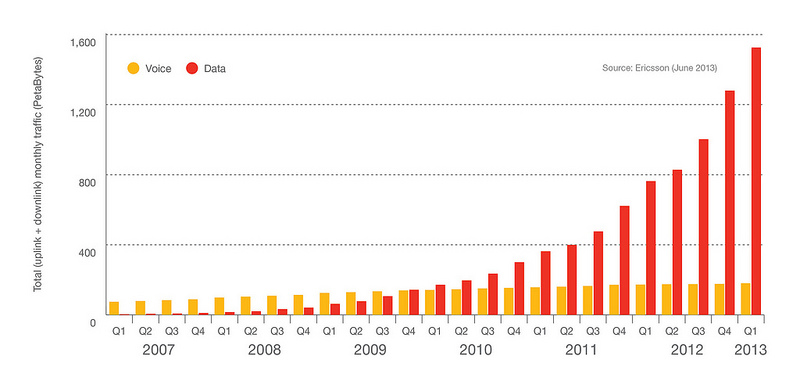
\includegraphics[width=0.8\textwidth]{ericsson/mob4.png}
  \caption{Глобальный общий трафик глоса и данных в мобильных сетях, 2007-2013 \cite{ericsson}}
  \label{img1:mob4}
\end{figure}






\clearpage





\section{Конвергенция фиксированный и мобильных сетей} \label{sect1_1}
В настоящее время большинство операторов сталкиваются с такими проблемами, как насыщение рынка, ценовое давление и необходимость снижения эксплуатационных затрат. Операторы фиксированной связи отмечают снижение доходов от предоставления традиционных голосовых услуг и потерю доли наземных линий доступа. Для операторов продолжилась эпоха слияний и поглощений, для вендоров - слияний, поглощений и поиска взаимовыгодных альянсов (когда продуктовые линейки и маркетинговые возможности компаний взаимовыгодно дополняют друг друга). По ряду технических и административных причин продолжился рост влияния на рынке компаний - системных интеграторов. Основными причинами этого называются расширение абонентской базы мобильной связи и развитие услуг передачи голоса через IP (Voice over IP - VoIP). В краткосрочной перспективе доходы провайдеров услуг фиксированной связи будут расти за счет доходов от услуг передачи данных IP, в частности, от широкополосных услуг для домашнего сектора.  Многие операторы мобильной связи столкнулись с проблемой замедления темпов роста базы частных абонентов и вынуждены были уделить серьезное внимание повышению доходности в других областях, таких как услуги передачи данных и услуги на корпоративном рынке. В качестве одного из решений перечисленных проблем появилась концепция конвергенции фиксированной и мобильной связи - Fixed Mobile Convergence (FMC), способствующей, с одной стороны, повышению доходов операторов, с другой - удовлетворению растущих требований конечных заказчиков, которые ориентированы на мобильные и IP-технологии. FMC будет способствовать принятию сетей нового поколения \cite{FMC}, в которых весь коммуникационный трафик использует IP.
Существует несколько способов предоставления FMC услуг, некоторые из которых более технологически интегрированы, чем другие. Есть менее развитые формы FMC использующие двухрежимные телефоны сотовый/Wi-Fi, которые не имеют функции handover или имею эту функцию, но не используют ее для передачи голоса или для доступа к широкополосной сети в домашних условиях. Также существуют услуги соединяющие мобильную и фиксированную сеть, но в которых технологически не происходит конвергенция, такие как предложение единого голосового и почтового ящика поверх фиксированных и мобильных сетей.
Концепция конвергенции фиксированных и мобильных сетей широка, многогранна и развивается. 


Концепция FMC состоит из трех основных уровней: конвергенция сетей; конвергенция услуг; конвергенция приложений \cite{IMS}.
\begin{enumerate}
\item Сетевая конвергенция. На уровне сетевой конвергенции обеспечивается снижение эксплуатационных расходов за счет конвергенции различных сетей фиксированной и мобильной связи в единую магистральную сеть IP/MPLS, поддерживающую широкий спектр методов доступа: традиционной телефонии, DSL, выделенных каналов, беспроводных сетей (WLAN) и сетей радиодоступа (RAN) в сетях операторов мобильной связи. Конвергенция магистрали и сетей доступа является наиболее очевидным и проработанным этапом процесса слияния фиксированных и мобильных платформ. Эта концепция охватывает и конвергенцию магистралей фиксированных и мобильных сетей, в том числе для передачи значительных объемов речевого трафика по той же магистрали IP, по которой доставляются широкополосные данные, услуги GPRS и UMTS, - так называемый перевод транзитного трафика на сеть IP. Для операторов мобильной связи конвергентные сети обычно начинаются переводом трафика SMS и MMS с традиционных платформ и сети сигнализации на сеть IP - это ускоряет конвергенцию протоколов сигнализации с IP. При передаче трафика сети радиодоступа 2.5G и 3G через оптимизированную сеть доступа IP сетевая конвергенция обеспечивает глубину проникновения вплоть до сети доступа оператора мобильной связи.


\item Конвергенция услуг. На уровне конвергенции услуг выполняются функции управления сессиями. Именно этот уровень делает возможным развертывание высокодоходных услуг нового поколения на основе IP, таких как мобильный доступ к данным, проведение аудио- и видеоконференций, передача голоса и мгновенный обмен сообщениями. Осведомленность о каждой сессии и контроль над ними обеспечивает доступность услуги на любом абонентском терминале и через любой метод доступа, позволяя переключаться между различными типами доступа без негативного воздействия на активные сессии. Кроме того, именно уровень конвергенции услуг гарантирует, что любой услуге IP выделяются соответствующие сетевые ресурсы, а любая услуга должным образом тарифицируется. Один из основных показателей функциональности конвергентной платформы - обеспечение непрерывности услуги при пересечении границы между фиксированной и мобильной сетями. Концепция непрерывности услуги достаточно специфична для каждой из областей - передачи голоса, передачи данных и передачи мультимедийного трафика. Однако такие технологии, как конвергентные голосовые устройства (телефоны, смартфоны, КПК, ноутбуки и т. д.), архитектуры конвергенции голосовых сессий и протоколы конвергенции сессий данных, являются связующим звеном между фиксированными и мобильными платформами. Другим ключевым элементом является осведомленность платформы, через которую доставляется услуга, о передаваемых сессиях и ее способность выполнять специфические действия по применению политик вне зависимости от местоположения участников сессии и их метода доступа, будь то проводной доступ по xDSL или мобильные данные в среде LTE. Конвергенция услуг - это тот основополагающий уровень, который в конечном счете обеспечивает потребителям удобство пользования услугами, выполняя незаметную для абонентов передачу сессий данных и голоса между наземным и беспроводным широкополосными доменами. При этом сеть динамически адаптирует свои политики по выделению ресурсов и обеспечению качества обслуживания, учитывая факт мобильности терминала и то, в какой среде передачи терминал находится в данный момент.

\item Конвергенция приложений. Уровень конвергенции приложений включает собственно услуги, с которыми операторы выходят на рынок и которые они собираются рекламировать в качестве конечного продукта. В частности, непрерывные услуги передачи данных, предоставляемые через любую сеть доступа, голосовые услуги для предприятий с двухрежимными терминалами (например, Wi-Fi/GSM) и т. д. Конвергенция приложений - это процесс доставки приложений через множество различных сред передачи в формате, учитывающем различие скоростей доступа, которые эти среды обеспечивают. Домен конвергентных приложений поддерживается и обеспечивается в основном функциональностью протокола SIP, учитывающего мобильность абонентов и динамичность их состояния (регистрации) на соответствующих серверах. Как один из примеров конвергентных приложений можно назвать одновременную доставку видеопотока на терминал 3G и персональный компьютер через сеть распространения контента из одного и того же сервисного центра. Более обобщенно, конвергенция приложений - это предоставление потребителям услуг голоса, данных и видео через все доступные типы сетей инновационными методами (WiFi, WiMax, LTE) . Реализация каждого из рассмотренных уровней обеспечивает значительные преимущества. Сетевая конвергенция создает возможности для экономии эксплуатационных расходов и капитальных затрат, конвергенция приложений - для предложения новых пакетов услуг и совершенствования маркетинга.

\end{enumerate}

Полная конвергенция - это совокупность всех перечисленных частей: сеть IP в качестве общей платформы, которая дает возможность предоставлять конвергентные приложения по конкурентоспособной цене и с непрерывностью услуги при пересечении границ сетей доступа. Побудительные причины для промышленного внедрения FMC различаются в разных сегментах рынка. FMC продолжает развиваться по отдельности по каждому из этих параметров. Поставщики услуг представляют решения, которые отвечают потребностям своих абонентов. Эти решения, по сути, следуют традиционному жизненному циклу модели разработки программного обеспечения, который постепенно добавляет функциональности.
FMC услуги представляет собой серьезную проблему для всех телекоммуникационных операторов в ближайшие несколько лет. Объединение разрозненных услуг по отдельным сетям стало рассматриваться как маркетинговый шаг, необходимый для поддержки заказчиков.



\subsection{IP-мультимедиа (IMS, IP Multimedia Subsystem)} \label{sect1_1_1}

В IP-сети сервисы - это обширный комплекс коммуникационных сервисов реального времени, подчиняющихся общим принципам архитектуры "клиент-сервер". Это такие сервисы как обмен мгновенными сообщениями (Instant Messaging, IM), мгновенную многоточечную связь (Push-to-Talk, PTT), NetMeeting, сервисы VoIP третьего поколения беспроводной связи. VoIP открывает дорогу услугам нового уровня, к которым относятся сервисы с учетом местоположения и присутствия в сети, мультимедийные сервисы, сотрудничество в реальном времени (collaboration) и многое другое.

Для реализации новых конвергентных услуг с гарантией качества обслуживания сеть должна соответствовать надежной сервисной архитектуре, подчиняющейся следующим требованиям:

\begin{itemize}
\item Отделение уровней транспорта и доступа от сервисного уровня (прозрачность доступа).
\item Управление сеансом связи, в ходе которого задействуются несколько сервисов связи реального времени.
\item Совместимость с имеющимися сервисами интеллектуальной сети (IN), к которым относятся: определение имени вызывающей стороны, бесплатный номер (800), переносимость локального номера, сервисы, соответствующие стандартам CAMEL, ANSI-41 и т.д.
\item Прозрачное взаимодействие с телефонными сетями (планы нумерации, сигнализация прохождения вызовов).
\item Конвергенция проводных и беспроводных сервисов.
\item Объединение голосовых услуг с сервисами реального времени (обмен мгновенными сообщениями).
\item Стандартизованные механизмы обмена пользовательской информацией между сервисами.
\item Стандартизованные механизмы аутентификации и биллинга конечных пользователей.
\item Стандартизованный, общий для всех сервисов графический пользовательский интерфейс.
\item Открытые стандартные интерфейсы и API для новых сервисов, разработанные сервис-провайдерами и третьими фирмами.
\end{itemize}
Архитектура IMS, удовлетворяющая изложенным выше требованиям, определена в стандартах 3GPP (3rd Generation Partnership Project) и Европейского института стандартов связи ETSI (рис. \ref{img:IMS}).
\begin{figure} [h]
  \center
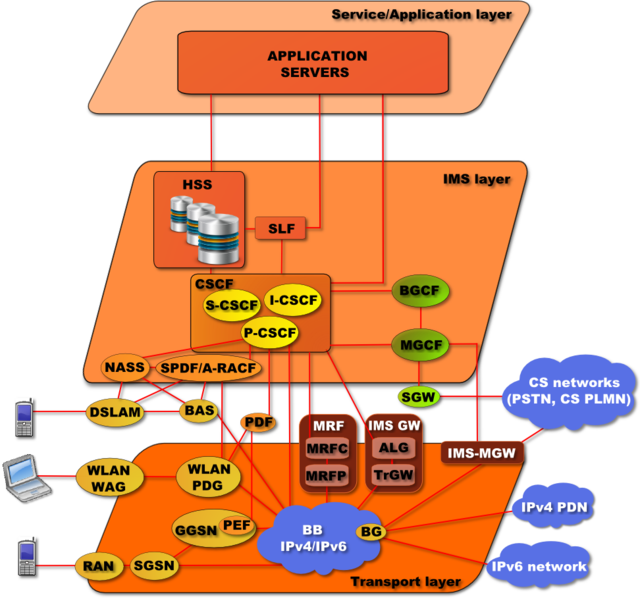
\includegraphics [width=0.95\textwidth] {Imsoverview-2.png}
  \caption{Архитектура IMS}
  \label{img:IMS}
\end{figure}

Унифицированная сервисная архитектура IMS поддерживает широкий спектр сервисов, основанных на гибкости протокола SIP (Session Initiation Protocol). IMS поддерживает множество серверов приложений, предоставляющих как обычные телефонные услуги, так и новые сервисы (обмен мгновенными сообщениями, мгновенная многоточечная связь, передача видеопотоков, обмен мультимедийными сообщениями и т.д.). Сервисная архитектура представляет собой набор логических функций, которые можно разделить на три уровня: уровень абонентских устройств и шлюзов, уровень управления сеансами и уровень приложений.

\textbf{Уровень абонентских устройств и транспорта.}

На этом уровне инициируется и терминируется сигнализация SIP, необходимая для установления сеансов и предоставления базовых услуг, таких как преобразование речи из аналоговой или цифровой формы в IP-пакеты с использованием протокола RTP (Realtime Transport Protocol). На этом уровне функционируют медиашлюзы, преобразующие базовые потоки VoIP в телефонный формат TDM. Медиасервер предоставляет различные медиасервисы, в том числе конференц-связь, воспроизведение оповещений, сбор тоновых сигналов, распознавание речи, синтез речи и т.п. Ресурсы медиасервера доступны всем приложениям, т.е. любое приложение (голосовая почта, бесплатный номер 800, интерактивные VXML-сервисы и т.д.), которому необходимо воспроизвести оповещение или получить цифры набранного номера, может использовать общий сервер. Медиасерверы также поддерживают и нетелефонные функции, например, тиражирование голосовых потоков для оказания сервиса мгновенной многоточечной связи (PTT). При использовании для различных сервисов общего пула медиасерверов отпадает необходимость в планировании и инжиниринге медиаресурсов для каждого отдельного приложения.


\textbf{Уровень управления вызовами и сеансами.}

На этом уровне располагается функция управления вызовами и сеансами CSCF (Call Session Control Function), которая регистрирует абонентские устройства и направляет сигнальные сообщения протокола SIP к соответствующим серверам приложений. Функция CSCF взаимодействует с уровнем транспорта и доступа для обеспечения качества обслуживания по всем сервисам. Уровень управления вызовами и сеансами включает сервер абонентских данных HSS (Home Subscriber Server), где централизованно хранятся уникальные сервисные профили всех абонентов. Профиль содержит текущую регистрационную информацию (например, IP-адрес), данные роуминга, данные по телефонным услугам (например, номер переадресации), данные по обмену мгновенными сообщениями (список абонентов), параметры голосовой почты (например, приветствия) и т.д. Централизованное хранение позволяет различным приложениям использовать эти данные для создания персональных справочников, информации о присутствии в сети абонентов различных категорий, а также совмещенных услуг. Централизация также существенно упрощает администрирование пользовательских данных и гарантирует однородное представление активных абонентов по всем сервисам.

На уровне управления вызовами и сеансами также располагается функция управления медиашлюзами MGCF (Media Gateway Control Function), которая обеспечивает взаимодействие сигнализации SIP с сигнализацией других медиашлюзов (например, H.248). Функция MGCF управляет распределением сеансов по множеству медиашлюзов, для медиасерверов это выполняется функцией MSFC (Media Server Function Control).

\textbf{Уровень серверов приложений.}

Этот уровень содержит серверы приложений, которые обеспечивают обслуживание конечных пользователей. Архитектура IMS и сигнализация SIP обеспечивают достаточную гибкость для поддержки разнообразных телефонных и других серверов приложений. Так, разработаны стандарты SIP для сервисов телефонии и сервисов IM.









\section{Анализ архитектуры беспроводной сети LTE} \label{sect1_2}
\subsection{Общая структура сети LTE} \label{sect1_2_1}
Сеть LTE состоит из двух важнейших компонентов \cite{lte}: сети радиодоступа E-UTRAN и базовой сети SAE (System Architecture Evolution) (рис. \ref{img:LTEscheme}).
\begin{figure} [h]
  \center
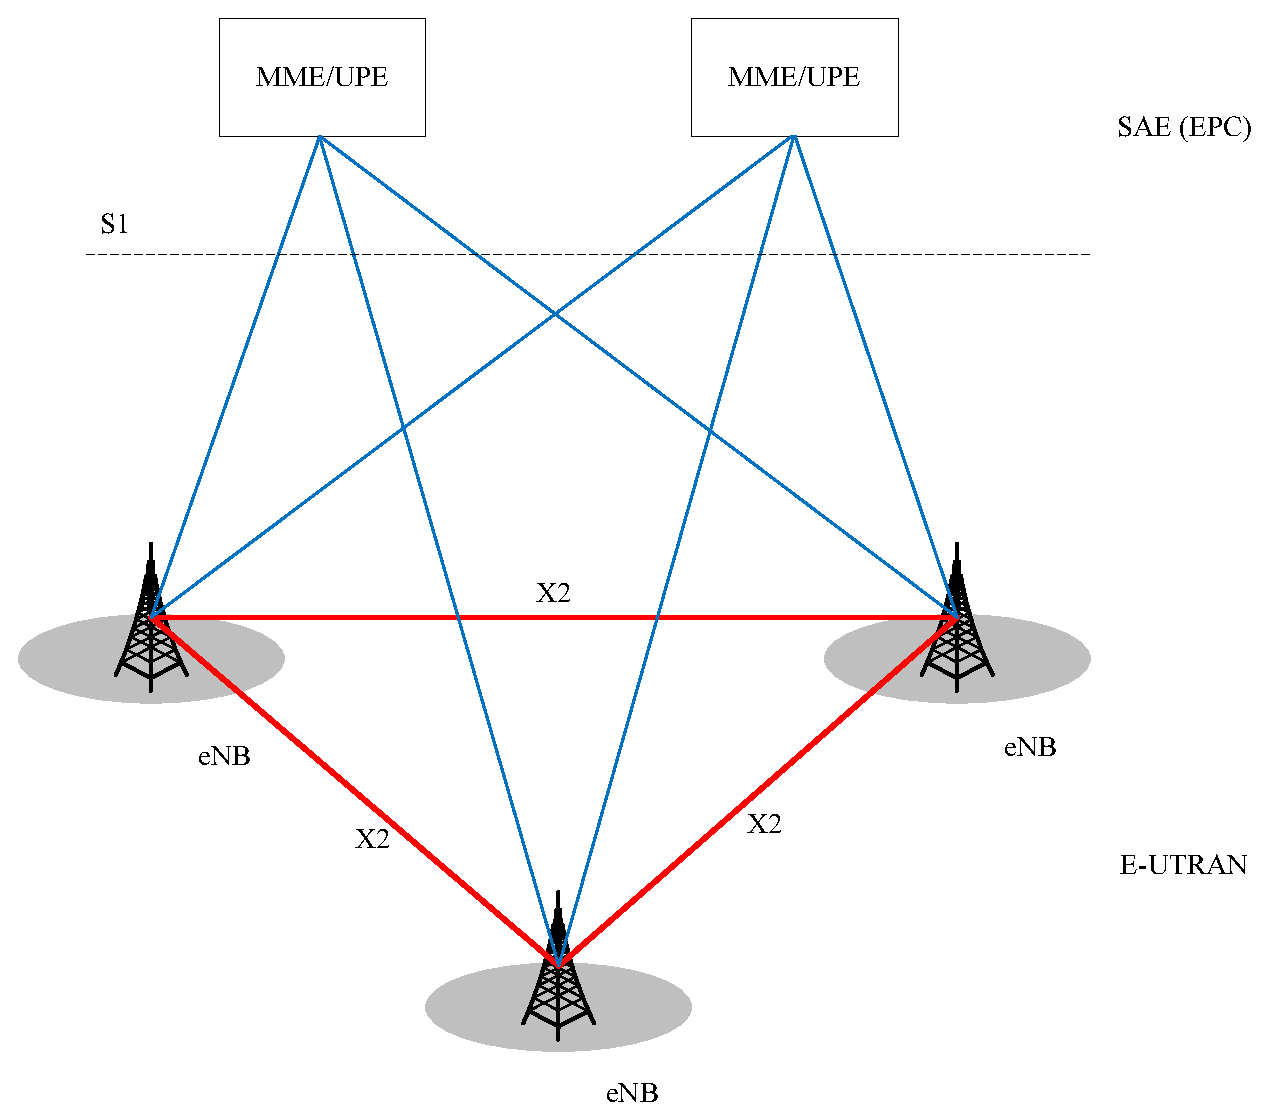
\includegraphics [width=0.8\textwidth] {LTEscheme.eps}
  \caption{Взаимодействие сети радиодоступа E-UTRAN и базовой сети SAE}
  \label{img:LTEscheme}
\end{figure}
Основными требованиями проекта 3GPP к сети SAE были: максимально возможное упрощение структуры сети и исключение дублирующих функций сетевых протоколов, характерных для систем UMTS.
Сети радиодоступа E-UTRAN рассмотрены в ряде технических спецификаций, согласно которым она состоит только из базовых станций eNB (evolved Node B). Базовые станции eNB являются элементами полносвязной сети E-UTRAN и соединены между собой по принципу каждый с каждым при помощи интерфейса X2. Интерфейс X2 поддерживает хендовер мобильного терминала в состоянии LTE\_ACTIVE. Каждая базовая станция имеет интерфейс S1 с базовой сетью SAE, построенный по принципу коммутации пакетов.
Базовая сеть SAE \cite{lte}, иногда называемая сетью EPC (Evolved Packet Core), содержит узлы MME/UPE, состоящие из логических элементов MME и UPE. Логический элемент MME (Mobility Management Entity) отвечает за решение задач управления мобильностью абонентского терминала и взаимодействует с базовыми станциями eNB сети E-UTRAN с помощью протоколов плоскости управления C-plane (интерфейс S1-C). Логический элемент UPE (User Plane Entity) отвечает за передачу данных пользователей согласно протоколам плоскости пользователя U-Plane и взаимодействует с eNB посредством интерфейса S1-U.
Благодаря интерфейсу S1 базовые станции соединены с несколькими узлами MME/UPE, что позволяет более гибко использовать сетевой ресурс. Такой интерфейс называют S1-flex.
Сеть LTE имеет следующие функциональные отличия от сети UMTS.

\begin{enumerate}
  \item Базовые станции eNB выполняют функции управления радиоресурсами RRM (Radio Resource Management): управление радиоканалами (Radio Bearer Control), управление доступом (Radio Admission Control), управление мобильностью (Connection Mobility Control), динамическое распределение ресурсов (Dynamic Resource Allocation). Таким образом, в сети радиодоступа E-UTRAN базовые станции eNB управляют протоколами радиоинтерфейса, комбинируя выполнение функций базовых станций Node В и большинства функций контроллера RNC сети UMTS.
  \item Сетевой элемент управления мобильностью MME отвечает за распределение сообщений вызова (paging) к базовым станциям eNB. Кроме того, MME управляет протоколами плоскости управления: назначения идентификаторов абонентских терминалов, обеспечения безопасности сети, проверки подлинности сообщений абонентов и управления роумингом.
  \item Сетевой элемент плоскости пользователя UPE выполняет сжатие заголовков IP-протоколов, шифрование потоков данных, терминацию пакетов данных плоскости пользователя, коммутацию пакетов данных при обеспечении мобильности пользователя. Кроме того, UPE управляет протоколами пользовательского уровня, например, хранением текущего статуса абонентского терминала (АТ), прерыванием состояния LET\_IDLE на уровне абонентских терминалов.
\end{enumerate}
Основные протоколы интерфейса S1 плоскостей C-plane и U-plane сети LTЕ представлены на рис. \ref{img:LTEinterface}.
\begin{figure} [h]
  \center
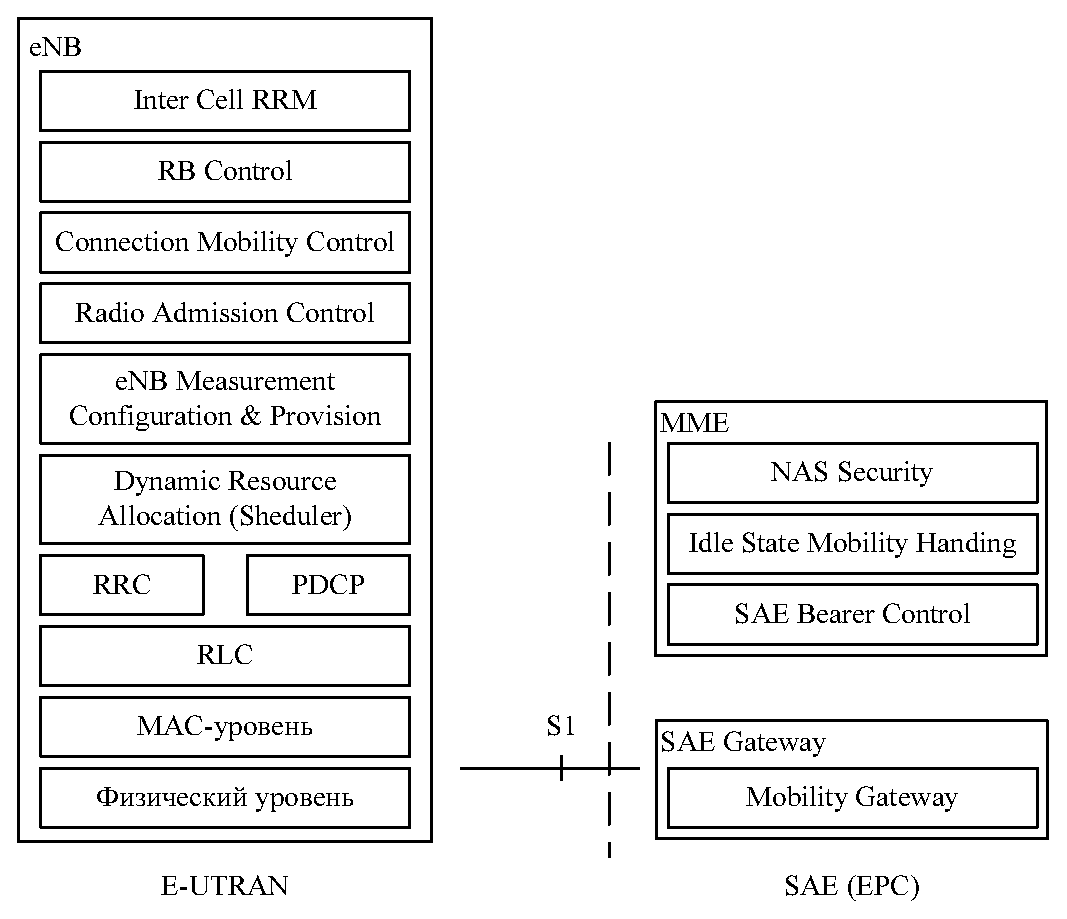
\includegraphics [width=0.6\textwidth] {LTEinterface.eps}
  \caption{Протоколы интерфейса S1 сети LTE}
  \label{img:LTEinterface}
\end{figure}
Одной из важнейших задач управления в сети LTE является максимально эффективное использование радиоресурсов. Данная задача решается с помощью совокупности функций управления радиоресурсами RRM (управление радиоресурсами сети E-UTRAN, управление службой передачи данных в радиоканале, управление мобильностью, управление доступом, динамическое распределение ресурсов) и с помощью протокола управления радиоресурсами RRC. 
Управление радиоресурсами сети E-UTRAN (Inter Cell RRM) обеспечивает управление ресурсами группы сот в целях повышения эффективности использования частотного спектра и минимизации помехового взаимного влияния абонентских терминалов и базовых станций, а также поддержку мобильности.
Управление службой передачи данных в радиоканале (RB Control) реализовано в базовых станциях eNB сети E-UTRAN и обеспечивает установление, поддержание и освобождение радиоканалов передачи данных с заданными параметрами в сети E-UTRAN. Основными задачами являются контроль и управление всеми активными сессиями передачи данных с учетом параметров качества услуг (QoS), выделение ресурсов для вновь активируемых сессий.
Управление мобильностью (Connection Mobility Control) позволяет выбирать обслуживающую базовую станцию eNB для мобильного терминала, передавать обслуживание мобильного терминала от одной базовой станции eNB (хэндовер) к другой. Выбор обслуживающей eNB осуществляется мобильным терминалом на основе собственных измерений в состоянии RRC\_CONNECTED и сравнения полученных измерений с установленными пороговыми значениями. Хэндовер реализован на основе анализа измерений как мобильного терминала, так и базовой станции eNB, а также текущей загрузки обслуживающей и соседних сот, политикой оператора по регулированию трафика.
Поддержку мобильности абонентского терминала в сети SAE обеспечивает логический элемент MME. Основными функциями MME являются:
\begin{itemize}
  \item Управление мобильностью абонентского терминала, находящегося в состоянии RRC\_IDLE (Idle State Mobility Handling).
  \item Управление безопасностью мобильной связи (NAS Security) в соответствии с протоколами, относящимися к группе протоколов «уровня без доступа» и обеспечивающими, например, аутентификацию пользователей, управление ключами шифрования данных.
  \item Управление службой передачи данных сети SAE (SAE Bearer Control).
\end{itemize}
Параметры функций управления радиоресурсами сети E-UTRAN (Inter
Cell RRM), управления службой передачи данных в радиоканале (RB Control) и управления мобильностью (Connection Mobility Control) могут быть кастомизированы в соответствии с требованиями оператора.
Основной задачей управления доступом (Radio Admission Control) является формирование решений о предоставлении доступа мобильному терминалу к сети E-UTRAN. Данная задача решается на основе многокритериального анализа загрузки сети радиодоступа, требований мобильного терминала к параметрам QoS.
Динамическое распределение ресурсов (Dynamic Resource Allocation; Scheduler) отвечает за планирование очередности передачи пакетов данных и позволяет динамически выделять и перераспределять ресурсы сети радиодоступа, включая канальные ресурсы, мощность излучения базовых станций, ресурсы буферизации при обработке пакетов данных с учетом параметров QoS.
Протокол управления радиоресурсами RRC плоскости С-plane обеспечивает:
\begin{itemize}
  \item Вещание служебной информации в соответствии с протоколами, относящимися к группам протоколов «уровня с доступом» и «уровня без доступа» (соответственно AS - Access Stratum и NAS - Non-Access Stratum).
  \item Пейджинг мобильного терминала.
  \item Установление, поддержание и закрытие RRC-соединений между абонентским терминалом и сетью E-UTRAN.
  \item Управление ключами шифрования.
  \item Установление, поддержание и закрытие служб передачи данных в радиоканале (Radio Bearers) типа «точка-точка» и «точка-многоточка» с заданными параметрами QoS.
  \item Мобильность абонентских терминалов.
\end{itemize}
Кроме того, протокол RRC обеспечивает выполнение ряда других функций.
Протокол сходимости пакетных данных PDCP (Packet Data Convergence Protocol) плоскостей U-plane и C-plane обеспечивает устранение избыточности (сжатие) служебной информации, объем которой может быть соизмерим с объемом полезной информации, передаваемой в пакетах данных, а также шифрование/дешифрование данных.
Протокол управления радиоканалом RLC (Radio Link Control) обеспечивает:
\begin{itemize}
  \item Сегментацию и компоновку пакетов данных протоколов более высокого уровня PDU (Protocol Data Unit) переменной длины в меньшие блоки полезной нагрузки PU (Packet Unit); размер блока PU определяется в соответствии со скоростью передачи информации в радиоканале.
  \item Конкатенцию (сочленение) коротких пакетов PDU верхнего уровня.
  \item Заполнение остатка поля данных блока PU, если сочленение неприемлемо.
  \item Передачу данных пользователя с подтверждением и неподтверждением приема в соответствии с параметрами QoS.
  \item Исправление ошибок методом повторной передачи (ARQ) пакетов данных.
  \item Сохранение на более высоком уровне порядка доставки пакетов PDU при передаче данных с подтверждением приема.
  \item Обнаружение дублирования пакетов PDU для доставки их на более высокий уровень только один раз.
  \item Управление скоростью передачи данных.
  \item Контроль порядковых номеров пакетов.
\end{itemize}


\subsection{Архитектура базовой сети SAE} \label{sect1_2_2}
Архитектура базовой сети SAE позволяет осуществлять дальнейшую эволюцию сетей 3G в направлении получения более высоких скоростей передачи данных, обеспечения низких задержек, а также оптимизации передачи данных на основе разнообразных технологий радиодоступа. Основным от личием базовой сети SAE от базовой сети системы UMTS является максимально упрощенная структура и отсутствие дублирующих функций сетевых протоколов.
Архитектура базовой сети SAE представляет собой PS-домен системы LTE, который предоставляет как голосовые услуги, так и всю совокупность IP-услуг на основе технологий пакетной коммутации данных. В основу построения базовой сети SAE положена концепция «все через IP» (all-IP или AIPN — All over IP Network) и то обстоятельство, что доступ к базовой сети SAE может осуществляться как через сети радиодоступа второго и третьего поколений (например, сети UTRAN, GERAN), так и через сети радиодоступа неевропейских технологий, не стандартизированные проектом 3GPP (сети He-3GPP), например, сети IEEE: Wi-Fi, WiMAX, а также через сети, использующие проводные IP-технологии (например, сети ADSL+, FTTH и др.).
Эталонная архитектура базовой сети SAE с указанием интерфейсов взаимодействия с внешними сетями показана на рис. \ref{img:SAEnetwork}. Согласно этой архитектуре функции протоколов плоскости управления узла SGSN сети UMTS становятся функциями элемента управления мобильностью MME. Функции контроллера RNC, которые не выполняет базовая станция eNB сети E-UTRAN, и функции протоколов плоскости пользователя узлов SGSN и GGSN реализуются модулем UPE и шлюзовым узлом «привязки» 3GPP Anchor сети SAE. Этот узел предназначен для присоединения сетей 2G/3G к сети LTE. В состав SAE входит также шлюзовый узел привязки SAE Anchor, который служит для присоединения к сети SAE сетей стандартов 3GPP (GSM/UMTS) и стандартов нe-3GPP (Wi-Fi и WiMAX). Узлы привязки 3GPP Anchor и SAE Anchor образуют единый узел привязки IASA (Inter Access System Anchor) для присоединения внешних IP-сетей.
Совокупность логических сетевых элементов MME/UPE, IASA, состоящего из узлов SAE Anchor и 3GPP Anchor (рис. \ref{img:SAEnetwork}), образует базовую пакетную сеть (Evolved Packet Core — ЕРС). Данные логические элементы рассматривались в основном на начальных стадиях разработки стандартов сети LTE. Более детальные исследования, направленные на практическую реализацию архитектуры ЕРС, определили новые сетевые элементы: обслуживающий шлюз S-GW (Serving GW) и шлюз взаимодействия с пакетными сетями P-GW (PDN GW), а также логический элемент MME, функционирующий отдельно от элемента UPE. Шлюзы S-GW и Р-GW физически могут быть реализованы в составе одного сетевого элемента AGW (Access GW).
Краткое описание основных интерфейсов сети SAE приведено в табл. \ref{SAEinterface}.
\begin{figure} [h]
  \center
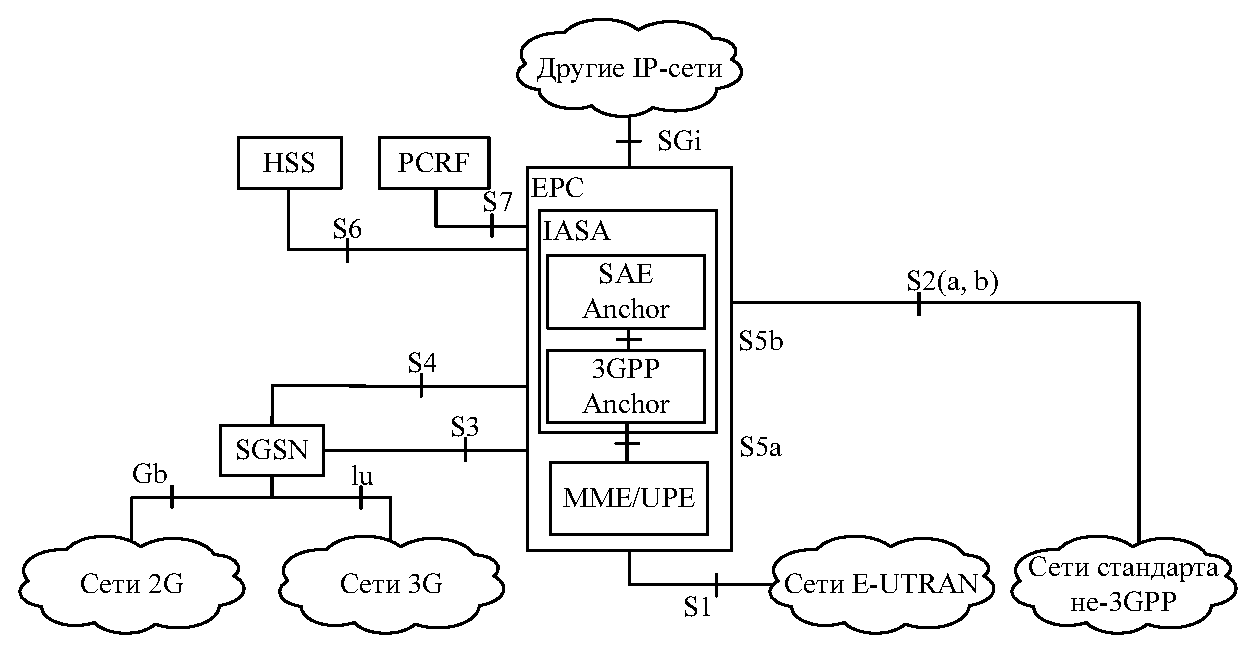
\includegraphics [width=0.95\textwidth] {SAEnetwork.eps}
  \caption{Эталонная архитектура базовой сети SAE}
  \label{img:SAEnetwork}
\end{figure}

\begin{table} [htbp]
  \centering
  \parbox{15cm}{\caption{Основные интерфейсы сети SAE}\label{SAEinterface}}
%  \begin{center}
  \begin{tabular}[t]{| p{3cm} || p{12cm}l |}
  \hline
  \hline
  Интерфейс & \centering  Описание интерфейса & \\
  \hline
  \hline
  S1 & \centering  Интерфейс, предоставляющий доступ к сети радиодоступа E-UTRAN для передачи данных протоколов плоскостей пользователя и управления. Позволяет иметь раздельную и комбинированную аппаратную реализацию элементов MME и UPE & \\
  \hline
  S2a & \centering Интерфейс между узлом IASA и фиксированными IP-сетями стандарта нe-3GPP. Обеспечивает передачу данных протоколов плоскости пользователя и поддержку функций управления и мобильности. Включает в себя интерфейсы S2a, S2b и S2c & \\
  \hline
  S3 & \centering Интерфейс между элементами MME/UPE и узлом SGSN. Обеспечивает управление межсетевым хэндовером абонентских терминалов в сетях E-UTRAN и UTRAN  & \\
  \hline
  S4 & \centering Интерфейс между узлом 3GPP Anchor и узлом SGSN. Обеспечивает передачу данных плоскости пользователя и поддержку функций управления и мобильности. Основан на интерфейсе Gn между узлами SGSN и GGSN сети UMTS  & \\
  \hline
  S5a & \centering Интерфейс между элементом MME/UPE и узлом 3GPP Anchor. Обеспечивает передачу данных протоколов плоскости пользователя и поддержку функций управления и мобильности  & \\
  \hline
  S5b & \centering Интерфейс между узлами 3GPP Anchor и SAE Anchor. Обеспечивает передачу данных протоколов плоскости пользователя и поддержку функций управления и мобильности   & \\
  \hline
  S6 & \centering Интерфейс, обеспечивающий доступ к домашней базе данных пользователей (HSS) для аутентификации и авторизации пользователей (интерфейс ААА) & \\
  \hline
  S7 & \centering Интерфейс, обеспечивающий управление установлением соединений с заданными параметрами QoS на основе политики сети и тарификацию (Policy and Charging Rules Function — PCRF)    & \\
  \hline
  SGi & \centering Интерфейс между узлом IASA и внешними сетями с пакетной передачей данных. Эти сети могут принадлежать как разным операторам, так и одному оператору сотовой связи для предоставления, например, услуг подсистемы IMS. Этот интерфейс основан на интерфейсе Gi между узлами GGSN и внешними IP-сетями  & \\
  \hline
  \hline
  \end{tabular}
%  \end{center}
\end{table}




\subsection{Формирование транспортного блока в LTE} \label{sect1_2_3}

На рис. \ref{img:frame_lte} изображено формирование кадра в сети LTE. Предположим что мы рассматриваем нисходящее направление соединения и предположим что соединение между UE и eNB уже было установленно. Данные с верхих уровней сначала поступают на PDCP (Packet data compression protocol) уровень. Этот уровень выполняет сжатие и шифрование данных и если необходимо устанавливает проверку на целосность. Далее данные передаются на RLC (LTE Radio Link Control) уровень, который объединяет PDCP PDUs в один RLC PDU.

RLC уровень объединит или сегментирует данные, поступающие от уровня PDCP в правильный размер блока и направит его на уровень МАС со своим собственным заголовком. Теперь MAC уровень выбирает схему модуляции и кодирования настраиваемую на физическом уровне. Теперь эти данные включенные в транспортный блок, должны быть переданы в 1 мс подкадре.

Теперь, рассмотрим количество бит, которые передаются в этом 1 мс интервале. Это зависит от MCS (схемы модуляции и кодирования) и количество ресурсных блоков назначены UE. Мы должны обратиться к таблице 7.1.7.1-1 и таблице 7.1.7.2.1-1 от \cite{3GPPTS36213}.

Давайте предположим, что eNB назначает MCS индекс 20 и 2 блока ресурсов (RB), на основании CQI и другую информацию для передачи по нисходящей линии связи через PDSCH (Physical Downlink Control Channel). Тогда необходимо взять значение TBS индекса равным 18, как показано в табл. \ref{TBindex}.

Узнав значение индекса TBS нам нужно обратиться к табл. \ref{TBS}, чтобы найти точный размер транспортного блока (только часть таблицы показан здесь в то время как для полного диапазона значений необходимо обратится к документу \cite{3GPPTS36213}).

Из табл. \ref{TBS} размер транспортного блока равен 776 бит для $I_{TBS}=18$ и  $N_{PRB}=2$. Проще говоря, кодовая скорость может быть определена как, насколько эффективно данные могут быть переданы в 1 мс транспортном блоке или, другими словами, она представляет собой отношение фактического количества битов, передаваемых к максимальному количеству битов, которое может передаваться в одном транспортном блоке.



\begin{equation}\label{eq:Reffective}
R_{effective}=\frac{TBS+CRC}{RE \times Q_{m}},
\end{equation}
\noindent где $TBS$ - размер транспортного блока взятый из табл. \ref{TBS}, $CRC$ - циклический избыточный код, $RE$ - ресурсы выделенные или PDSCH или PUSCH, $Q_{m}$ - используемая  схема модуляции, где $\{2,4,6\}$ соответсвуют QPSK, 16QAM и 64QAM.

Пока нам известно $TBS$, $CRC$, $Q_{m}$ и необходимо вычислить $RE$. В нашем случае, предположим, что 10\% $RE$ предназначены для каналов управления (PDCCH и PHICH), то:

$TBS=776$,

$CRC=24$,

$RE=2(RB) \times 12($поднесущих$) \times 7 ($предположим 7 OFDM символа$) \times 2 ($слота на кадр$) \times 0.9 ($ранее предположенные 10\% на управление$)= 302$,

$Q_{m}=6$.

Таким образом $R_{effective}=\frac{776+24}{302 \times 6}=0.4$.

%\clearpage
\begin{figure} [h]
  \center
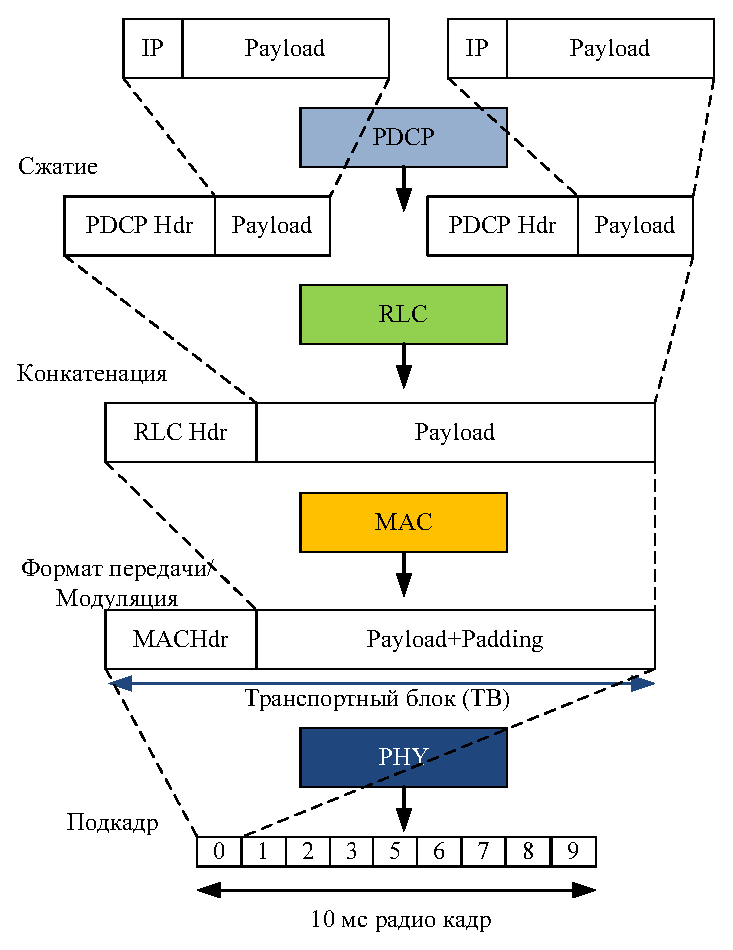
\includegraphics{frame_lte.eps}
  \caption{Формироваие транспортного блока (TB) в LTE}
  \label{img:frame_lte}
\end{figure}





\clearpage

\begin{table} [htb]
  \centering
\parbox{15cm}{\caption{Модуляция и TBS индексы для PDSCH}\label{TBindex}}
    \begin{tabular}{|l|l|l|}
    \hline
     MCS индекс ($I_{MCS}$) &  Порядок модуляции ($Qm$) &  TBS индекс ($I_{TBS}$)    \\ \hline
    0      & 2    & 0         \\ \hline
    1      & 2    & 1         \\ \hline
    2      & 2    & 2         \\ \hline
    3      & 2    & 3         \\ \hline
    4      & 2    & 4         \\ \hline
    5      & 2    & 5         \\ \hline
    6      & 2    & 6         \\ \hline
    7      & 2    & 7         \\ \hline
    8      & 2    & 8         \\ \hline
    9      & 2    & 9         \\ \hline
    10     & 4    & 9         \\ \hline
    11     & 4    & 10        \\ \hline
    12     & 4    & 11        \\ \hline
    13     & 4    & 12        \\ \hline
    14     & 4    & 13        \\ \hline
    15     & 4    & 14        \\ \hline
    16     & 4    & 15        \\ \hline
    17     & 6    & 15        \\ \hline
    18     & 6    & 16        \\ \hline
    19     & 6    & 17        \\ \hline
    20     & 6    & 18        \\ \hline
    21     & 6    & 19        \\ \hline
    22     & 6    & 20        \\ \hline
    23     & 6    & 21        \\ \hline
    24     & 6    & 22        \\ \hline
    25     & 6    & 23        \\ \hline
    26     & 6    & 24        \\ \hline
    27     & 6    & 25        \\ \hline
    28     & 6    & 26        \\ \hline
    29     & 2    &  reserved \\
    30     & 4    & ~         \\
    31     & 6    & ~         \\ \hline
    \end{tabular}
\end{table}

\clearpage

\begin{table} [htb]
  \centering
\parbox{15cm}{\caption{Размеры Транспортных блоков (TBS)}\label{TBS}}
\begin{center}
    \begin{tabular}{|l||l|l|l|l|l|l|l|l|l|l|}
\hline
& \multicolumn{10}{c|}{$N_{PRB}$} \\
\cline{2-11}
\raisebox{1.5ex}[0cm][0cm]{$I_{TBS}$}
& 1   & 2   & 3    & 4    & 5    & 6    & 7    & 8    & 9    & 10   \\
\hline
\hline
    0    & 16  & 32  & 56   & 88   & 120  & 152  & 176  & 208  & 224  & 256  \\ \hline
    1    & 24  & 56  & 88   & 144  & 176  & 208  & 224  & 256  & 328  & 344  \\ \hline
    2    & 32  & 72  & 144  & 176  & 208  & 256  & 296  & 328  & 376  & 424  \\ \hline
    3    & 40  & 104 & 176  & 208  & 256  & 328  & 392  & 440  & 504  & 568  \\ \hline
    4    & 56  & 120 & 208  & 256  & 328  & 408  & 488  & 552  & 632  & 696  \\ \hline
    5    & 72  & 144 & 224  & 328  & 424  & 504  & 600  & 680  & 776  & 872  \\ \hline
    6    & 328 & 176 & 256  & 392  & 504  & 600  & 712  & 808  & 936  & 1032 \\ \hline
    7    & 104 & 224 & 328  & 472  & 584  & 712  & 840  & 968  & 1096 & 1224 \\ \hline
    8    & 120 & 256 & 392  & 536  & 680  & 808  & 968  & 1096 & 1256 & 1384 \\ \hline
    9    & 136 & 296 & 456  & 616  & 776  & 936  & 1096 & 1256 & 1416 & 1544 \\ \hline
    10   & 144 & 328 & 504  & 680  & 872  & 1032 & 1224 & 1384 & 1544 & 1736 \\ \hline
    11   & 176 & 376 & 584  & 776  & 1000 & 1192 & 1384 & 1608 & 1800 & 2024 \\ \hline
    12   & 208 & 440 & 680  & 904  & 1128 & 1352 & 1608 & 1800 & 2024 & 2280 \\ \hline
    13   & 224 & 488 & 744  & 1000 & 1256 & 1544 & 1800 & 2024 & 2280 & 2536 \\ \hline
    14   & 256 & 552 & 840  & 1128 & 1416 & 1736 & 1992 & 2280 & 2600 & 2856 \\ \hline
    15   & 280 & 600 & 904  & 1224 & 1544 & 1800 & 2152 & 2472 & 2728 & 3112 \\ \hline
    16   & 328 & 632 & 968  & 1288 & 1608 & 1928 & 2280 & 2600 & 2984 & 3240 \\ \hline
    17   & 336 & 696 & 1064 & 1416 & 1800 & 2152 & 2536 & 2856 & 3240 & 3624 \\ \hline
    18   & 376 & 776 & 1160 & 1544 & 1992 & 2344 & 2792 & 3112 & 3624 & 4008 \\ \hline
    19   & 408 & 840 & 1288 & 1736 & 2152 & 2600 & 2984 & 3496 & 3880 & 4264 \\ \hline
    20   & 440 & 904 & 1384 & 1864 & 2344 & 2792 & 3240 & 3752 & 4136 & 4584 \\ \hline    
    \end{tabular}
\end{center}
\end{table}


\section{Обзор концепции потоковых агентов} \label{sect1_3}
При передаче мультимедийной информации по комбинированным сетям с учетом различных механизмов распространения с различными технологиями, важным является выполнение требований по качеству предоставления мультимедийной информации пользователю.
При этом важными являются такие характеристики: задержка, джиттер, число потерянных и поврежденных пакетов. Как показывает практика наибольшие потери качественных характеристик происходит на границах операторских сетей и сетей с различными механизмами распространения.
Возникает необходимость установки соответствующих агентов, обеспечивающих мониторинг на том или ином промежутке сети. Вместе с тем от числа и места этих агентов существенно зависит качество мониторинга.
Потоковый агент (ПА) это агент, который находится на базовой станции на пересечении проводной и беспроводной сети (рис. \ref{img:SA}). Агент просматривает и распознает поток, исследуя заголовки RTP. Агент периодически посылает статистические и обратные сообщения в реальном времени на отправляющий сервер. Статистические обратные связи помогают отправителю проследить проводное состояние сети, что существенно для выполнения надлежащего контроля над перегрузками. С другой стороны, потоковый агент отправляет обратные сообщения в реальном времени, такие как подтверждение пакетов (ACKs), что говорит отправителю о прибытии каждого пакета к агенту корректно и вовремя.


\begin{figure} [h]
  \center
\includegraphics [width=0.95\textwidth] {SA.eps}
  \caption{Использование ПА}
  \label{img:SA}
\end{figure}

Блок формирования находится перед ПА и ограничивает объем отправляемых сообщений, чтобы он не был больше чем полоса пропускания беспроводной сети, храня пакеты, ожидающие фрагментацию и передачу на более низкий уровень. Если состояние беспроводной сети плохое, то число повторных передач будет расти, заставляя увеличиваться очередь пакетов. Блок формирования реагирует на заполненность очереди, отбрасывая пакеты до прибытия их к агенту.

ПА позволяет выполнять множество функций для улучшения качества предоставления мультимедийных услуг:
\begin{itemize}
\item ПА предоставляет дополнительную обратную связь для контент сервера с границы между проводной  и беспроводной частью сети \cite{SAdouble_feedback}.
\item ПА дает возможность определить место пакетной ошибки \cite{SAdouble_feedback}, что позваляет корректно реагировать на потери и задержки в сети.
\item Предварительное отбрасывание пакетов, которые передаются сверх возможностей беспроводной сети.
\item Ретрансляция на прикладном уровне позволяет уменьшить  пакетные искажения  для приложений не восприимчивых к задержке \cite{SArateOpt, SArealtime}.
\item Прямая коррекция ошибок позволяет уменьшить битовые искажения для приложений восприимчивых к задержке \cite{SArateOpt, SArealtime}.
\end{itemize}




\section{Архитектура имитационной модели LTE в NS3} \label{sect1_4}
Обзор имитационной модели LTE-EPC изображен на рис. \ref{img:LTEEPC}. Состоит из двух основных компонентов:
\begin{itemize}
  \item Модель LTE. Эта модель включает LTE радио стек протоколов (RRC, PDCP, RLC, MAC, PHY). Эти объекты полностью находятся на UE и eNB узлах.
  \item Модель EPC. Эта модель включает в себя основные сетевые интерфейсы, протоколы и объекты. Эти объекты и протоколы находятся на S-GW, P-GW и MME узлах и частично на eNB узлах. 
\end{itemize}

\begin{figure} [h]
  \center
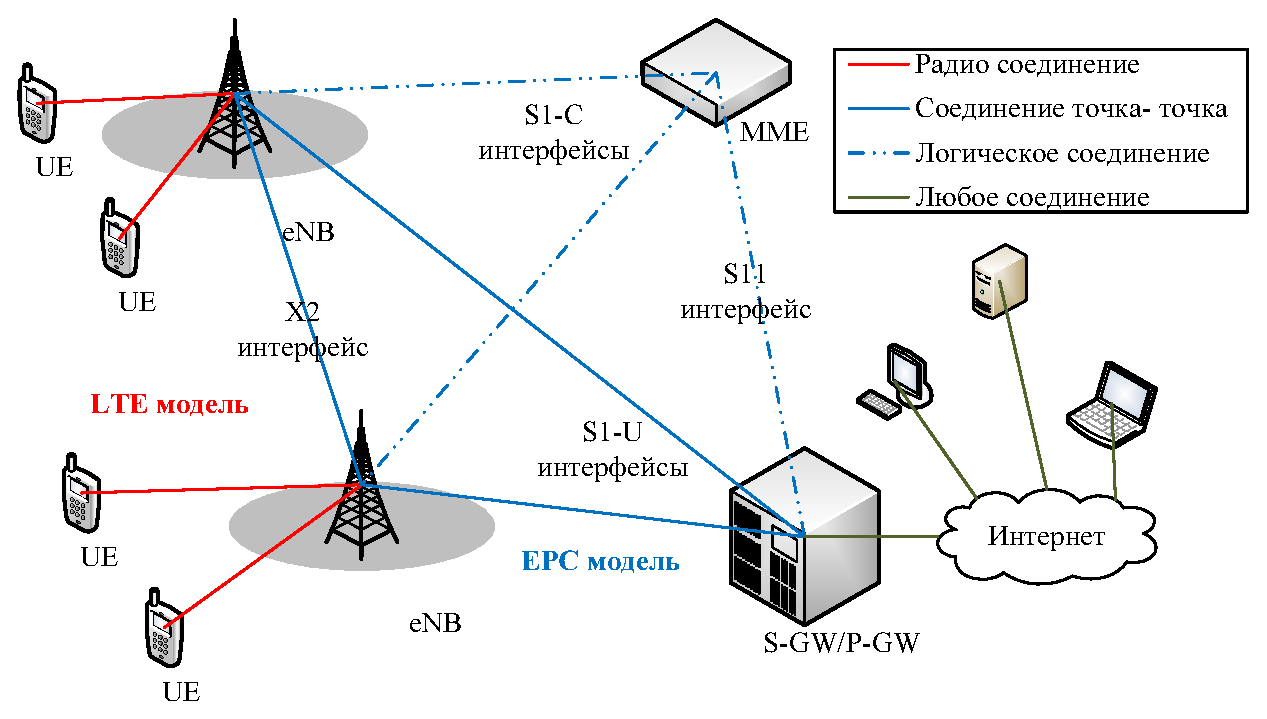
\includegraphics [width=0.95\textwidth] {LTEEPC.eps}
  \caption{Обзор имитационной модели LTE-EPC \cite{LteSimDoc}}
  \label{img:LTEEPC}
\end{figure}



\subsection{Архитектура LTE модели} \label{sect1_4_1}
LTE модель была разработана для поддержки оценки следующих аспектов системы LTE:
\begin{itemize}
  \item Управление радио ресурсами.
  \item Пакетная обработка на основе QoS.
  \item Внутрисистемные помехи между сотами.
  \item Динамический спектральный доступ
\end{itemize}


Архитектура физического и канального уровня для модели узла UE представлена на рис. \ref{img:UEPHY} и для модели узла eNB представлена на рис \ref{img:eNBPHY}.
\begin{figure} [h]
  \center
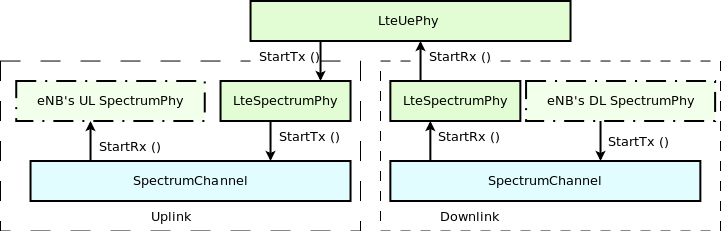
\includegraphics [width=0.95\textwidth] {UEPHY.png}
  \caption{Архитектура физического и канального уровня для модели UE \cite{LteSimDoc}}
  \label{img:UEPHY}
\end{figure}

\begin{figure} [h]
  \center
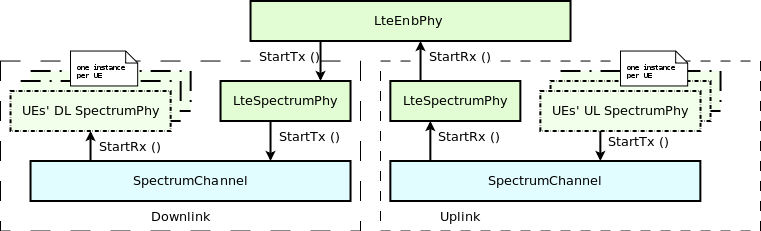
\includegraphics [width=0.95\textwidth] {eNBPHY.png}
  \caption{Архитектура физического и канального уровня для модели eNB \cite{LteSimDoc}}
  \label{img:eNBPHY}
\end{figure}


\subsection{Архитектура EPC модели} \label{sect1_4_2}
Модели EPC обеспечивает средства для моделирования сквозного IP соединения по верх LTE модели. В частности, поддерживает соединение нескольких UE с интернетом через сеть радиодоступа с несколькими узлами eNB, подключенными к одному SGW/PGW узлу. Эта топология сети изображен на рис \ref{img:LTEEPCdata}.
Основное внимание в модели ЕРС в настоящее время сфокусировано на плоскости данных EPC. Чтобы понять архитектуру этой модели, мы сначала посмотрим на рис \ref{img:LTEEPCdata}, где представлен сквозной LTE-EPC стек протоколов таким образом каким это реализовано в симуляторе. Из рисунка видно, что самые большие упрощения введены в модели ЕРС для плоскости данных, является включение функций SGW и PGW в один узел SGW / PGW, который устраняет необходимость S5 или S8 интерфейсов, определенных в 3GPP . С другой стороны, все уровни протокола S1-U и протокола радиосвязи LTE стек, указанные в 3GPP, присутствуют.

\begin{figure} [h]
  \center
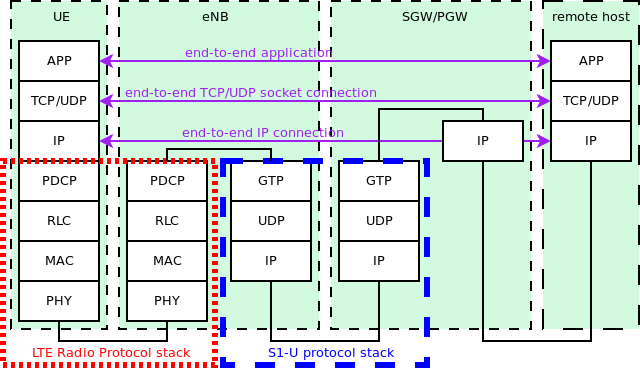
\includegraphics [width=0.95\textwidth] {LTEEPCdata.png}
  \caption{Архитектура физического и канального уровня для модели eNB \cite{LteSimDoc}}
  \label{img:LTEEPCdata}
\end{figure}

Как показано на рисунке, существует два различный уровня IP-сети. Первый это сквозной уровень, который обеспечивает сквозное подключение к пользователям; этот слой включает UE, PGW и удаленный хост (в том числе возможные интернет маршрутизаторы и хосты между ними), но не включать eNB. По умолчанию, UE присваивается публичный адрес IPv4 из 7.0.0.0/8 сети и PGW присваивается адрес 7.0.0.1, который используется всеми UE, в качестве шлюза для доступа в Интернет.
Второй слой IP сетей является ePC локальной сетью. Которая включает в себя все узлы ENB и SGW/PGW узел. Эта сеть реализован в виде набора соединений точка-точка, которые соединяют каждый eNB с SGW/PGW узлом, таким образом, SGW/PGW имеет набор устройств точка-точка, каждый из которых обеспечивает подключение к другому eNB. По умолчанию, подсети 10.xyz/30 присваивается каждому соединению точка-точка.
Как указано в 3GPP, сквозные IP соединения являются тунелями через локальную EPC IP сеть с использованием GTP/UDP/IP. Далее рассмотрим как это туннелирование реализовано в модели ЕРС. Объяснение сделано путем обсуждения сквозного потока пакетов данных.

Для начала, рассмотрим случай нисходящей линии связи, который изображен на рис \ref{img:DownloadUE}. IPv4 пакеты нисходящей линии связи генерируются от общего удаленного хоста и адресуются к одному из устройств UE. Интернет маршрутизация будет заботиться о пересылке пакета на публичный сетевой интерфейс NetDevice узла SGW/PGW, который подключен к Интернету (этот интерфейс Gi в соответствии с 3GPP терминологии). SGW/PGW имеет сетевой интерфейс VirtualNetDevice которому присваивается IP-адрес шлюза для подсети UE, следовательно, правило статической маршрутизации приведет к тому, что входящий пакет из Интернета будут проходить через VirtualNetDevice. Это сетевое устройство начинает GTP/UDP/IP туннельную процедуру, путем пересылки пакетов на выделенное приложение на узле SGW/PGW, которое называется EpcSgwPgwApplication. Это приложение выполняет следующие операции:
\begin{figure} [h]
  \center
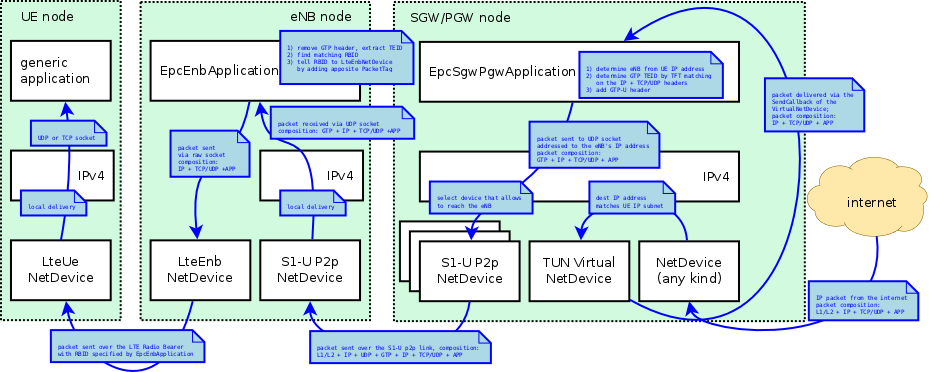
\includegraphics [width=0.95\textwidth] {DownloadUE.png}
  \caption{Поток данных нисходящей линии связи между интернетом и узлом UE \cite{LteSimDoc}}
  \label{img:DownloadUE}
\end{figure}

\begin{enumerate}
  \item Определяет eNB узел, к которому присоединен UE, смотря на IP-адрес назначения (который является адресом UE).
  \item Классифицирует пакеты, используя шаблоны транспортных потоков (TFT - Traffic Flow Templates), чтобы идентифицировать, какому ePS каналу он принадлежит. ePS каналы имеют карту соответсвия к S1-U каналам, так что эта операция возвращает идентификатор TEID (GTP-U Tunnel Endpoint Identifier), к которому принадлежит данный пакет.
  \item Добавляет соответствующие GTP-U-заголовки к пакету.
  \item Отправляет пакет через UDP-сокет к S1-U P2P NetDevice, адресуя к eNB, с которым соединен UE.
\end{enumerate}
Как следствие, пакес со сквозным IP заголовком с добавленными IP, UDP и GTP заголовками отправляется S1 соединение к eNB, где он принимается и доставляется локально (в качестве адреса назначения подставляется приватный адрес eNB). Локальный процесс доставки отправит пакет через UDP сокет к выделенному приложению EpcEnbApplication. Это приложение выполняет следующие операции:
\begin{enumerate}
  \item Удаляет заголовок GTP и извлекает TEID, который содержится в нем.
  \item Используя на взаимно-однозначное соответствие между S1-U каналами и радио каналами (который является 3GPP требованием), определяет идентификатор радиоканала (RBID -Radio Bearer ID), к которому принадлежит данный пакет.
  \item Записывает RBID в выделенном тег под названием LteRadioBearerTag, который добавляется к пакету.
  \item Пересылает пакет к приложению LteEnbNetDevice eNB узла через raw сокет.
\end{enumerate}
Следует отметить, что в этот момент, внешним заголовком пакета является сквозной IP заголовок, поскольку IP/UDP/GTP заголовки S1 стека протоколов уже были удалены. После приема пакета от EpcEnbApplication, LteEnbNetDevice будет извлекать RBID из LteRadioBearerTag, и на основе RBID определит экземпляр радиоканала (и соответствующие PDCP и RLC экземпляры протокола), которые затем используются для передачи пакета к UE через радиоинтерфейс LTE. В конце, приложение LteUeNetDevice узла UE получит пакет и доставит его локально через IP стек протоколов, которые в свою очередь доставит его к приложению на узле UE, которое является конечной точкой нисходящей линии связи.

В случае восходящего соединения, показанном на рис. \ref{img:UploadUE} , IP пакеты создаются приложением внутри UE, и передается локальным стеком протоколов TCP / IP к приложению LteUeNetDevice узла UE. LteUeNetDevice затем выполняет следующие операции:
\begin{enumerate}
  \item Классифицирует пакет, испоьзуя TFT, и определяет радиоканал, к которому принадлежит пакет (и соответствующие RBID).
  \item Определяет соответствующий экземпляр протокола PDCP, который является точкой входа LTE радио стеком протоколов для этого пакета.
  \item Посылает пакет к eNB через LTE радио стек протоколов.
\end{enumerate}
eNB принимает пакет через его сетевой интерфейс LteEnbNetDevice. Поскольку существует один экземпляр протокола PDCP и RLC для каждого радиоканала, LteEnbNetDevice способен определить RBID пакета. Это RBID затем записывается в LteRadioBearerTag, который добавляется к пакету. LteEnbNetDevice затем пересылает пакет EpcEnbApplication через сокет пакета.
При получении пакета EpcEnbApplication выполняет следующие операции:
\begin{enumerate}
  \item Извлекает RBID из тега LteRadioBearerTag в пакете.
  \item Определяет соответствующий EPS канал и GTP-U TEID за счет использования на взаимно-однозначное соответствие между S1-U каналами и радиоканалами.
  \item Добавляет GTP-U заголовок пакета, в том числе TEID, который был определен ранее.
  \item Посылает пакет на SGW/PGW узел через UDP сокет подключенный к S1-U сетевому точка-точка устройству.
\end{enumerate}

В этот момент пакет содержит S1-U IP, UDP и GTP заголовки в дополнение к первоначальному сквозному IP заголовку. Когда пакет поступает на соответствующий S1-U P2P NetDevice на узле SGW/PGW, он доставляется локально. Локальный процесс доставки направляет пакет к EpcSgwPgwApplication через соответствующий UDP сокет. EpcSgwPgwApplication затем удаляет заголовок GTP и пересылает пакет VirtualNetDevice. На данный момент, внешним заголовком пакета является сквозной IP заголовок. Следовательно, если адрес назначения в этот заголовке является удаленным узлом в интернете, пакет отправляется в интернет через соответствующие сетевое устройство NetDevice на узле SGW/PGW. В случае, если пакет адресован другому UE, IP стек SGW/PGW перенаправит пакет снова к сетевому устройству VirtualNetDevice, и пакет будет проходить через процесс доставки через нисходящее соединение для того, чтобы достичь пункта назначения UE.

\begin{figure} [h]
  \center
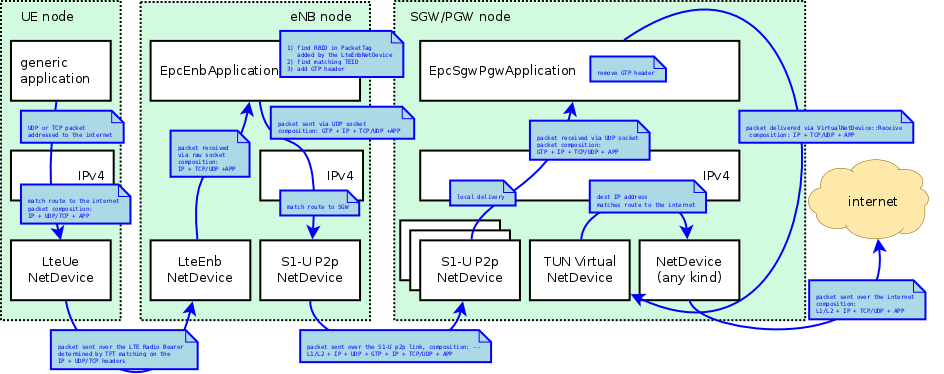
\includegraphics [width=0.95\textwidth] {UploadUE.png}
  \caption{Поток данных восходящей линии связи между узлом UE и интернетом \cite{LteSimDoc}}
  \label{img:UploadUE}
\end{figure}



\clearpage




